\documentclass[10pt]{beamer}

\usetheme[progressbar=frametitle]{metropolis}
\usepackage{appendixnumberbeamer}
\definecolor{maincolor}{RGB}{35, 55, 58}
\usepackage{booktabs}
\usepackage[scale=2]{ccicons}
\usepackage{tcolorbox}
\tcbuselibrary{theorems}
\usepackage{pgfplots}
\usepgfplotslibrary{dateplot}
\usepackage{xspace}
\usepackage{tikz-cd}
\setbeamercovered{transparent}
\newcommand{\themename}{\textbf{\textsc{metropolis}}\xspace}
\usepackage{graphicx}
\usepackage{subcaption}
\graphicspath{ {./images/} }




% {{{
\def\sh{\mathcal}                   % sheaf font
\def\bb{\mathbb}                    % bold font
\def\cat{\mathtt}                   % category font
\def\leq{\leqslant}                 % <=
\def\geq{\geqslant}                 % >=
\def\setmin{-}                      % set minus
\def\rad{\mathfrak{r}}              % radical
\def\nilrad{\mathfrak{N}}           % nilradical
\def\emp{\varnothing}               % empty set
\def\vphi{\phi}                     % for switching \phi and \varphi, change if needed
\def\HH{\mathrm{H}}                 % cohomology H
\def\CHH{\check{\HH}}               % Čech cohomology H
\def\RR{\mathrm{R}}                 % right derived R
\def\LL{\mathrm{L}}                 % left derived L
\def\dual#1{{#1}^\v}              % dual
\def\v{\smash{\scalebox{.8}[1.4]{\rotatebox{90}{\guilsinglleft}}}}
\def\kres{k}                        % residue field k
\def\C{\cat{C}}                     % category C
\def\op{^\cat{op}}                  % opposite category
\def\Set{\cat{Set}}                 % category of sets
\def\CHom{\cat{Hom}}                % functor category
\def\supertilde{{\,\widetilde{\,}\,}}   % use \supertilde instead of ^\sim
\def\GL{\bb{GL}}
\def\Q{\bb{Q}}
\def\Z{\bb{Z}}
\def\R{\bb{R}}
\def\C{\bb{C}}
\def\O{\sh{O}}
\def\G{\bb{G}}
\def\P{\bb{P}}
\def\bbGamma{\boldsymbol\Gamma}
\def\red{\mathrm{red}}
\def\rg{\operatorname{rg}}
\def\gr{\operatorname{gr}}
\def\Gr{\operatorname{Gr}}
\def\Sym{\operatorname{Sym}}
\def\Hom{\operatorname{Hom}}
\def\Proj{\operatorname{Proj}}
\def\Tor{\operatorname{Tor}}
\def\Ext{\operatorname{Ext}}
\def\Supp{\operatorname{Supp}}
\def\Ker{\operatorname{Ker}}
\def\Im{\operatorname{Im}}
\def\Coker{\operatorname{Coker}}
\def\Spec{\operatorname{Spec}}
\def\Spf{\operatorname{Spf}}
\def\grad{\operatorname{grad}}
\def\dimc{\operatorname{dimc}}
\def\codim{\operatorname{codim}}
\def\id{\operatorname{id}}
\def\Der{\operatorname{Der}}
\def\Diff{\operatorname{Diff}}
\def\Hyp{\operatorname{Hyp}}
\def\Tr{\operatorname{Tr}}
% }}}

\newtcbtheorem{colordef}{Definition} {theorem style = plain, colback=maincolor!30!white, coltitle=black, colframe=black, fonttitle = \upshape\bfseries, fontupper=\itshape}{th}

\newtcbtheorem[no counter]{colorthm}{Theorem} {theorem style = plain, colback=maincolor!30!white, coltitle=black, colframe=white, fonttitle = \upshape\bfseries, fontupper=\itshape}{th}

\newtcbtheorem[no counter]{colorconj}{Conjecture} {theorem style = plain, colback=maincolor!30!white, coltitle=black, colframe=white, fonttitle = \upshape\bfseries, fontupper=\itshape}{conj}

\newtcbtheorem{constructionbox}{Construction} {theorem style = plain, colback=maincolor!30!white, coltitle=black, colframe=black, fonttitle = \upshape\bfseries, fontupper=\upshape}{th}

%\usepackage{floatrow}

\title{Derived categories of coherent sheaves}
% \date{\today}
\date{}
\author{Bogdan Simeonov}
% \titlegraphic{\hfill\includegraphics[height=1.5cm]{logo.pdf}}

\begin{document}

\maketitle
%Computer Project?

\begin{frame}{Overview}
    \begin{itemize}
        \pause
        \item The derived category of a variety \pause
        \item The Kuznetsov component and its geometric meaning \pause
        \item Cubic fourfolds containing a plane 
    \end{itemize}
 
\end{frame}

\begin{frame}[fragile]{The cubic fourfold}
    Let $X\subset \P^5$ be the zero locus of a degree $3$ polynomial. We can compare its Hodge diamond to that of a K3 surface: \pause

                            %\captionsetup{justification=centering}
                        %   \begin{center}
                                %\hfill
                                
                        %       \begin{minipage}[t]{0.4\textwidth}
                        %       \centering
                        %           \begin{figure}[H]
                        %           \begin{tikzcd}[ampersand replacement=\&, row sep=0.10em, column sep=0.10em]
                        %               \\
                        %               \\
                        %               \\
                        %               \\
                        %               \\
                        %               \\
                        %               \\
                        %               \\
                        %               \\
                        %               \\
                        %               \\
                        %               \\
                        %               \\
                        %              \\
                        %              \\
                        %               \\
                        %               \\
                        %               \\
                        %               \\
                        %               \\
                        %               \\
                        %               \\
                        %               \\
                        %               \\
                        %               \\
                        %               \\
                        %               \\
                        %               \\
                        %               \\
                        %               \\
                        %               \&   \& 1  \&   \&   \\
                        %               \& 0 \&    \& 0 \&   \\
                        %           1 \&   \& 20 \&   \& 1 \\
                        %               \& 0 \&    \& 0 \&   \\
                        %               \&   \& 1  \&   \& 
                        %           \end{tikzcd}
                        %
                        %            \caption*{Hodge diamond of K3 surface} \label{fig: MonFun2}
                        %            \end{figure}
                        %        \end{minipage}
                        %        %\captionsetup{justification=centering}
                        %        \begin{minipage}[t]{0.4\textwidth}
                        %        \centering
                        %            \begin{figure}[H]
                        %            \begin{tikzcd}[ampersand replacement=\&, row sep=0.10em, column sep=0.10em]
                        %                \&   \&   \&   \& 1  \&   \&   \&   \&   \\
                        %                \&   \&   \& 0 \&    \& 0 \&   \&   \&   \\
                        %                \&   \& 0 \&   \& 1  \&   \& 0 \&   \&   \\
                        %                \& 0 \&   \& 0 \&    \& 0 \&   \& 0 \&   \\
                        %            0 \&   \& 1 \&   \& 21 \&   \& 1 \&   \& 0 \\
                        %                \& 0 \&   \& 0 \&    \& 0 \&   \& 0 \&   \\
                        %               \&   \& 0 \&   \& 1  \&   \& 0 \&   \&   \\
                        %                \&   \&   \& 0 \&    \& 0 \&   \&   \&   \\
                        %                \&   \&   \&   \& 1  \&   \&   \&   \& 
                        %            \end{tikzcd}
                        %            \centering\caption*{\,\,\,\,\,\,\,\,Hodge diamond of X} \label{fig: MonFun3}
                        %            \end{figure}
                        %        \end{minipage}
                            %\hfill
                            %\null
                        %    \end{center}
\begin{figure}
    \centering
    \begin{minipage}{0.45\textwidth}
        \centering
        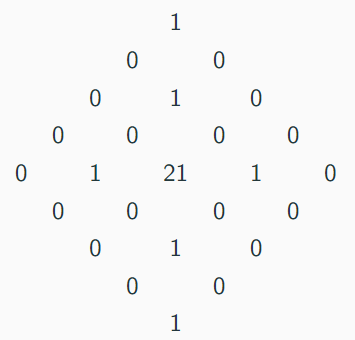
\includegraphics[width=0.9\textwidth]{CubicFourfoldHodgeDiamond.png} % first figure itself
        \caption*{Cubic fourfold}
    \end{minipage}\hfill
    \begin{minipage}{0.45\textwidth}
        \centering
        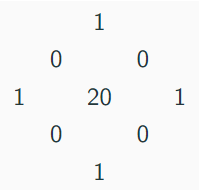
\includegraphics[width=0.4\textwidth]{K3diamond} % second figure itself
        \caption*{K3 surface}
    \end{minipage}
\end{figure}\pause

If we take the primitive cohomology of the cubic fourfold, we get something that looks exactly like a K3 surface! However, we run into a problem: the two have different signatures!
\end{frame}

\begin{frame}{The cubic fourfold}
    The solution is to pass to codimension one subspaces which have the same signature $(19,2)$. On the K3 side, we just take the primitive part. In many cases (the special cubic fourfolds) we can find a class $T\in H^{2,2}(X,\mathbb{Z})$ that allows us to pass to the orthogonal complement.

    \begin{colorthm}{Hasset}{}
        
    \end{colorthm}
    
\end{frame}








    

\end{document}
